\documentclass{standalone}
\usepackage{tikz}
\usepackage{pgfplots}
\pgfplotsset{compat=1.18}
\usetikzlibrary{calc}
\usetikzlibrary{arrows.meta}

\begin{document}
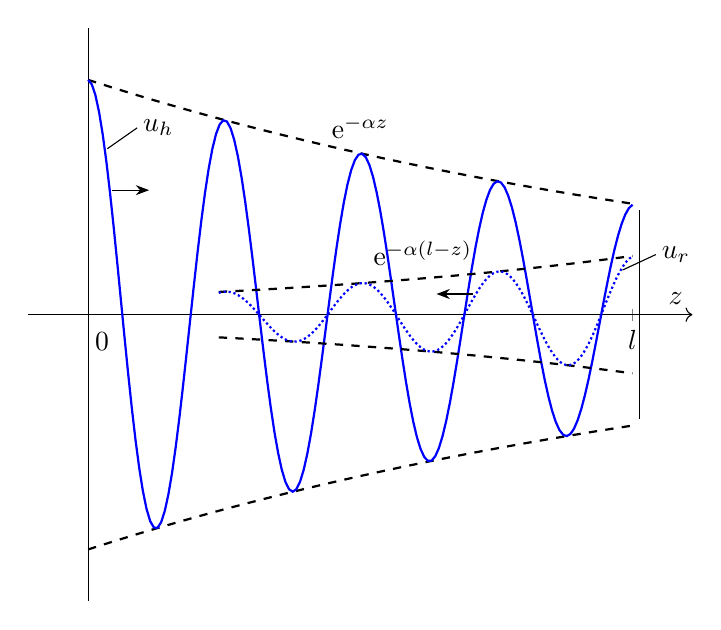
\begin{tikzpicture}
\begin{axis}[
scale only axis,
xmin=0, xmax=25, ymin=-1, ymax=1,
axis x line=center,
axis y line=left,
axis lines=middle, % Place axes in the middle
xlabel={$z$}, % Label for x-axis
%      xlabel style={at={(axis description cs:1,0.45)}},
ylabel={}, % Label for y-axis
samples=150, % Number of samples for smooth curve
yticklabels={},
ytick=\empty,
xtick={25},
xticklabels={$l$},
enlargelimits=0.11, % Ensure axes extend slightly beyond data
y axis line style={-}, % No arrows on y axis
x axis line style={->}, % Arrow on axes
separate axis lines,
]

% manually place 0 tickmark
\node[below=3pt, xshift=5pt] at (axis cs:0,0) {0};

% hinlaufende Welle
\addplot[dashed, thick, domain=0:25] {exp(-0.03*x)} node [pos=0.5, above, inner sep=5pt] {$\mathrm{e}^{- \alpha z}$}
node[inner sep=2pt, right] (P1) {};
\addplot[dashed, thick, domain=0:25] {-exp(-0.03*x)} node[inner sep=2pt, right] (P2) {};
\addplot[blue, thick, domain=0:25] {exp(-0.03*x)*cos(deg(x))} node[pos=0.03, inner sep=0] (H1) {} node[pos=0.04, inner
sep=0] (H2) {};
\draw (H1) -- +(35:0.5cm) node[right, inner sep=2pt] {$u_{h}$};
\draw[-Stealth] (H2) -- +(0:0.5cm);

% ruecklaufende Welle
\addplot[dashed, thick, domain=6:25] {0.25*exp(-0.05*(25-x))} node [pos=0.5, above, inner sep=4pt, xshift=-1pt]
{$\mathrm{e}^{-
\alpha (l-z)}$};
\addplot[dashed, thick, domain=6:25] {-0.25*exp(-0.05*(25-x))};
\addplot[blue, thick, densely dotted, domain=6:25] {0.25*exp(-0.05*(25-x))*cos(deg(x))} node[pos=0.97, inner sep=0]
(R1) {} node[pos=0.62, inner sep=0] (R2) {};
\draw (R1) -- +(25:0.5cm) node[right, inner sep=2pt] {$u_{r}$};
\draw[-Stealth] (R2) -- +(0:-0.5cm);

\draw (P1) -- (P2);

\end{axis}

\end{tikzpicture}

\end{document}